\documentclass{article}
\usepackage[a4paper]{geometry}
\usepackage{graphicx}

\title{Misure Elettroniche}
\author{Francesco Pio Cecca}
\date{November 2021}

\begin{document}

\maketitle

\section{La Misurazione Delle Grandezze Fisiche}

La misurazione è un processo che mette in relazione l'insieme “reale” degli eventi fisici e quello 
“astratto” dei numeri. Lo scopo della misurazione è quello di poter fornire una descrizione rigorosa 
e non soggettiva del fenomeno e permettere l'esecuzione di processi decisionali. 
Vantaggi delle misure elettroniche: 
\begin{itemize}
    \item Amplificabilità diretta 
    \item Trasmissibilità a distanza 
    \item Registrabilità 
    \item Elaborabilità 
\end{itemize} 

I trasduttori sono dispositivi in grado di fornire in uscita un segnale elettrico il cui valore è funzione 
dell'andamento di una grandezza fisica non elettrica presente in ingresso: permettono quindi di 
eseguire misurazioni su grandezze fisiche di tipo disparato mediante le tecniche e gli strumenti 
delle misure elettriche.

\subsection{Definizioni dalla norma UNI 4546}

\textbf{Misura}: informazione costituita da un numero, una incertezza ed una unità di misura assegnata a 
rappresentare un parametro in un determinato stato del sistema. 
Quindi la corrispondenza tra insieme degli eventi fisici e quello di numeri non è 1 a 1, ma ad ogni 
grandezza associo un intervallo di numeri, di ampiezza pari alla incertezza e centrato sul valore 
della grandezza da misurare (misurando). \\ \\
\textbf{Grandezza}: Ogni quantità, proprietà, condizione usata per descrivere fenomeni e valutabile in 
termini di 
unità di misura. Il termine "grandezza" viene usato in senso generale pertanto esso non deve 
essere usato per indicare l'oggetto di una misurazione, cioè il misurando, ma un suo parametro. \\ \\ 
Le grandezze misurabili sono classificabili in 5 categorie principali: 
\begin{itemize}
    \item GRANDEZZA DI TIPO NUMERALE: grandezza che riguarda la numerazione di oggetti o eventi individuati singolarmente, i cui valori sono espressi da numeri interi positivi (es: numero di esami sostenuti) 
    \item GRANDEZZA DI TIPO RAZIONALE: ogni grandezza i cui valori sono espressi da numeri razionali, rappresentanti il rapporto tra la grandezza misurata ed una determinata grandezza della stessa specie assunta come u.d.m. (esempio: frequenza di lavoro dei telefoni cellulari GSM) 
    \item GRANDEZZA DI TIPO STRUMENTALE: ogni grandezza i cui valori sono espressi come corrispondenza biunivoca con punti di scale convenzionalmente interpolabili (esempio: temperatura in C o in F)
    \item GRANDEZZA DI TIPO SELETTIVO: ogni grandezza riguardante il riconoscimento della appartenenza ad una certa classe (intensità del terremoto secondo la scala Mercalli) 
    \item GRANDEZZA DI TIPO COMPLESSO: ogni grandezza i cui valori sono espressi mediante un insieme ordinato di numeri relativi, presupponendo un sistema di riferimento (posizione di un punto materiale in un sistema di coordinate x, y, z) 
\end{itemize}
\textbf{Paramento}: Ogni grandezza pertinente a un "sistema" alla quale è necessario assegnare valori per descrivere il sistema stesso, la sua evoluzione e/o le sue interazioni con altri sistemi e con l'ambiente. \\ \\
\textbf{Segnale}: modificazione dello stato di un sistema usata per ottenere, elaborare e/o trasmettere un'informazione. \\ \\
\textbf{Rumore o disturbo}: variazione della grandezza costituente il supporto di un segnale non correlata all'informazione da esso trasmessa. \\ \\
\textbf{Unità di misura (u.d.m.)}: termine di riferimento adottato, per convenzione, per confrontare una grandezza con altre della stessa specie. \\ \\
\textbf{Sistema di unità di misura}: /insieme organico di definizioni, tra loro collegate, di u.d.m. pertinenti a grandezze di specie diverse:
\begin{itemize}
    \item SISTEMI DI U.D.M. NON COERENTI: un sistema di u.d.m. non coerente definisce una u.d.m. per ciascuna grandezza. 
    \item SISTEMI DI U.D.M. ASSOLUTI (O COERENTI): un sistema di u.d.m. assoluto definisce, in modo indipendente tra loro, solamente alcune u.d.m., che vengono dette "di base" (o "fondamentali"). Esse vengono scelte in maniera opportuna e le altre u.d.m. devono potere essere ricavate da quelle di base mediante leggi di coordinamento note. Le u.d.m. ricavate da quelle di base vengono dette "unità derivate". 
    
    \end{itemize}
    
\subsection{Il sistema SI e le unità di misura}
\textbf{Sistema Internazionale}: Sistema assoluto di u.d.m. proposto da Giovanni Giorgi e basato sulla definizione di 7 u.d.m. di base: massa, tempo, lunghezza, intensità di corrente elettrica, quantità di sostanza, temperatura, intensità luminosa. \\
Dalle u.d.m. di base si possono ricavare, mediante le "leggi di coordinamento", le unità di misura di tutte le altre grandezze: frequenza, forza, pressione, lavoro etc. \\
\textbf{Campioni delle u.d.m}: elementi materiali oppure fenomeni fisici utilizzati per rendere “tangibile” la unità di misura (es: ampere e la bilancia elettrodinamica). \\
\newpage
Requisiti di un campione:
\begin{itemize}
    \item ASSOLUTO: il suo valore non dipende dal luogo in cui è conservato 
    \item STABILE: il suo valore non deve variare nel tempo e Riproducibile e disseminabile: deve essere possibile realizzare delle copie fedeli da 
    conservare in luoghi diversi 

\end{itemize}

\subsection{Gli istituti metrologici e i campioni delle U.D.M}

\textbf{Istituti metrologici primari}: realizzano e conservano i campioni primari delle diverse nazioni \\ \\
\textbf{Massa}
\begin{itemize}
    \item U.d.m. della massa: kilogrammo. \\ 
    Si è convenzionalmente stabilito che un certo blocco di platino iridio avesse massa unitaria. La massa di quest’ultimo è quindi la u.d.m. della massa.
    \item Campione di massa: il campione di massa è un campone materiale. Il campione primario di massa è costituito dal blocco di platino/iridio che ha incertezza nulla. Le sue copie costituiscono i campioni primari dei diversi stati: essi hanno incertezze non nulle (1/1049). 
\end{itemize} 
\textbf{Secondo}
\begin{itemize}
    \item U.d.m. del tempo: secondo. \\
    Il secondo è il tempo corrispondente a 9 192 631 770 periodi della radiazione corrispondente alla transizione iperfina da (F=4, MF=0) a (F=3, MF=0) dell'atomo di cesio 133 non perturbata da campi esterni. 
    \item Il campione di tempo è un campione naturale. Il campione reale è implementato da un orologio atomico al cesio 133, con incertezza nell'ordine di 1014-13. 
\end{itemize}
\textbf{Metro}
\begin{itemize}
    \item U.d.m. della lunghezza: metro. \\
    Il metro è la distanza percorsa, nel vuoto, dalla luce in un intervallo di tempo pari a 1/299 792 458 secondi. 
    \item Il campione di lunghezza è un campione naturale implementato da strumenti la cui incertezza, derivata dal processo usato per definire l’udm, è di 1041-9. 
\end{itemize} 
\textbf{Intensità della corrente elettrica }
\begin{itemize}
    \item U.d.m. dell'intensità della corrente elettrica: ampere 
    L’ampere è l'intensità di una corrente elettrica costante che, in due conduttori paralleli, retillinei, di lunghezza infinita, sezione circolare trascurabile e posti ad 1 metro di distanza 
    nel vuoto, produrrebbe fra questi conduttori una forza di 2x104-7 newton per metro di lunghezza. 
    \item Campione di intensità di corrente: bilancia elettrodinamica. I campioni avevano incertezze maggiori di quelle raggiunte con campioni f.e.m. e di resistenza. 
\end{itemize}
\textbf{Forza elettromotrice }
\begin{itemize}
    \item Campione f.e.m. ad effetto Josephson: la giunzione piombo-niobio, se irradiata, diventa superconduttore locale a intervalli regolari di tensione, a temperature prossime a 0 K. 
    Siccome AV=(h/2e) x 2f, dipende solo dalla frequenza f, posso misurare corrente e tensione del metallo, aumentando la corrente da 0 e contare i tratti a V costante. Ho ottenuto la tensione sul 
    metallo dalla frequenza della radiazione. 
\end{itemize}
\textbf{Resistenza} 
\begin{itemize}
     \item Campione R a effetto Hall quantistico: prendo una basetta in materiale semiconduttore, con uno spessore di pochi mm, investita da un campo magnetico con una induzione B > 10 T ad una temperatura di circa 4 kelvin. Si sviluppa una tensione ai capi in base alla corrente imposta: V=(h/ne42) x 1= Rkx1, dove Rk è la costante di Von Klitzing che viene usata come 
    campione per la resistenza. 
    \end{itemize}
\textbf{Campioni secondari}: Un campione secondario è uno strumento destinato ad essere usato come campione, che ottiene la propria riferibilità da un altro campione, tramite una taratura \\ \\
\textbf{Forza elettromotrice}
\begin{itemize}
    \item Pila di Weston: Vengono periodicamente tarate per confronto con il campione di Josephson 
e servono per poter disporre di un campione pratico da usare con relativa comodità. \\
Funziona sul principio dell’elettrolisi (il solfato di cadmio è l’elettrolita).\\ Eroga correnti 
estremamente deboli e per un limitato periodo di tempo. 
    \item Campione a diodo zener: sfrutta il fenomeno naturale della conduzione di corrente nei 
semiconduttori polarizzati; usa la caratteristica lineare 1/V nella regione di breakdown nei 
diodi Zener. 
\end{itemize}
\textbf{Resistenza }
\begin{itemize}
    \item Campioni di resistenza in lega metallica: utilizzano leghe metalliche a basso coefficiente di 
dipendenza dalla temperatura (manganina, evanhom, karma).
    \item Campione di resistenza: resistore a quattro morsetti.
\end{itemize}
\textbf{Tempo}
\begin{itemize}
    \item Oscillatore al quarzo 
    \item Oscillatore a rete RC
\end{itemize}
\subsection{Incertezza di misura}
\textbf{Incertezza della misura UNI4546}: intorno limitato del valore di un parametro, 
corrispondente agli elementi della fascia di valore individuata dalla misurazione. \\
L'incertezza di una misura finita è un intorno simmetrico del valore e si indica con un 
numero + i associato alla stessa unità di misura usata per esso (valore), o con altra notazione 
dalla quale questo numero può essere ricavato. L’incertezza di una misura è pari a 2i.\\ \\
\textbf{Incertezza assoluta}: rappresenta l'ampiezza dell'intervallo centrato sul valore indicato g entro cui 
si considera compreso il valore del misurando.\\ Viene indicata col simbolo $\Delta g$ ed è dotata di 
dimensioni omogenee alla grandezza sotto misura: 
\begin{equation}
    \Delta g=\pm i
\end{equation}
\textbf{Incertezza relativa}: rappresenta il rapporto fra i valori dell'incertezza assoluta $\Delta g$ e del valore del 
parametro.\\ È adimensionale e viene indicata con:
\begin{equation}
    \frac{\Delta g}{g}=\pm \frac{i}{g}
\end{equation}
\textbf{Incertezza percentuale}: valore dell'incertezza relativa moltiplicato per 100. \\ \\
\textbf{Cause della incertezza}:
\begin{itemize}
    \item incertezza del campione utilizzato 
    \item l’imprecisione costruttive dello strumento usato per eseguire il rapporto fra il parametro 
incognito ed il campione 
    \item la perturbazione allo stato del sistema apportato dallo strumento
    \item i disturbi e i rumori che si sovrappongono al misurando. 
Le prime 3 sono cause sistematiche, l’ultima è una causa aleatoria. 
\end{itemize}
Per ridurre l'incertezza possiamo utilizzare diversi procedimenti, a seconda del tipo di causa: 
\begin{itemize}
    \item tarature periodiche dello strumento (per errori sistematici) 
    \item non eseguire misure durante il riscaldamento degli strumenti
    \item eseguire una media di più misurazioni
    \item tenere conto della perturbazione dello stato del sistema vedendo i parametri di 
quest’ultimo e dello strumento.
\end{itemize}
\subsection{Propagazione dell'incertezza nelle misure indirette}
Quando non è possibile misurare direttamente il parametro di cui si cerca la misura, la 
misurazione si ottiene attraverso la misurazione di altri parametri dai quali il misurando dipende 
attraverso leggi conosciute: si parla in questo caso di “misure indirette” in quanto la misurazione 
ha luogo non sull’incognita, ma su altre grandezze delle quali l’incognita è funzione. \\\\
\textbf{Funzioni di singola variabile } \\
se il legame fra l’incognita g ed il parametro misurato a viene espresso dalla generica 
funzione f (g=f(a)), il valore del misurando go si ottiene calcolando il valore della funzione 
in corrispondenza del valore misurato (indicato con il pedice 0) di a: 
\begin{equation}
    g_{0}=f(a)\vert_{a=a_{0}}
\end{equation}
Per individuare l'incertezza della misura indiretta si può utilizzare lo sviluppo in serie della 
funzione f sostituendo all'incremento della variabile indipendente il valore della sua 
incertezza assoluta.\\ Se l’incertezza assoluta ha un valore basso tale da poter essere 
trascurato e il valore della derivata prima della f in a0 non è nullo, allora si può 
approssimare utilizzando la forma linearizzata:
\begin{equation}
    \Delta g \cong \frac{df(a)}{da}\vert_{a=a_{0}}\Delta a
\end{equation}
\textbf{Funzione di due o più variabili }\\
Se il legame fra l’incognita g e le grandezze a e b viene epresso dalla generica funzione f 
(g=f(a,b)), il valore del misurando si ottiene calcolando il valore della funzione in 
corrispondenza dei valori misurati (indicati col pedice 0) delle due grandezze a e b
\begin{equation}
    g_{0}=f(a,b)\vert_{a=a_{0},b=b_{0}}
\end{equation}
Anche in questo caso, si può individuare l'incertezza attraverso lo sviluppo in serie della 
funzione, tenendo conto di 2 ipotesi restrittive: 
\begin{enumerate}
    \item Le incertezze di a e b non sono correlate 
    \item Le incertezze hanno valore talmente piccolo da poter essere trattate come 
infinitesimi 
\end{enumerate}
L'incertezza assoluta può essere ricavata dallo sviluppo in serie della funzione f(a,b) 
nell’intorno del punto (a0, bO) in cui gli incrementi delle variabili a e b vengono sostituiti 
dalle rispettive incertezze assolute e tutti i termini vengono presi col segno positivo.\\ Se 
non si annullano le derivate parziali prime, la espressione della incertezza può essere 
troncata ai termini del primo ordine approssimando la funzione con la sua forma 
linearizzata:
\begin{equation}
    \Delta g \cong \pm \vert \frac{\partial f(a,b)}{\partial a}|_{a=a_{0},b=b_{0}} \Delta a+|\frac{\partial f(a,b)}{\partial b}|_{a=a_{0},b=b_{0}}
\end{equation}
\textbf{Regole pratiche per la stima dell’incertezza nelle misure derivate attraverso le operazioni elementari}
\begin{equation}
    g=a+b \Rightarrow \Delta g = \pm |\Delta a|+|\Delta b|
\end{equation}
\begin{equation}
    g=a-b \Rightarrow \Delta g = \pm |\Delta a|+|\Delta b|
\end{equation}
\begin{equation}
    g=ab \Rightarrow \Delta g = \pm |\frac{\Delta a}{a}|+|\frac{\Delta b}{b}|
\end{equation}
\begin{equation}
    g=\frac{a}{b} \Rightarrow \Delta g = \pm |\frac{\Delta a}{a}|+|\frac{\Delta b}{b}|
\end{equation}
\textbf{Cifre significative } \\
$g = 123,45689$ volt $\Delta g = \pm 0,002$ volt \\
L'incertezza assoluta è dunque 0,004 volt (4mV), pertanto si ha $123,455 V < g < 1234,459 V$  
\begin{center}
    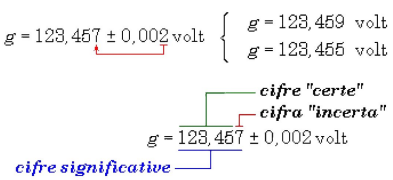
\includegraphics[scale=0.9]{Cifre Significative.png}
\end{center}
Le cifre significative del valore di una misura sono tutte quelle “certe” e la prima “incerta".\\\\
\textbf{Errori di perturbazione e di consumo }\\
Ad un esame superficiale si potrebbe pensare che il circuito che descrive la misurazione della 
tensione di un segnale sia il seguente:
\begin{center}
    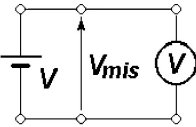
\includegraphics[scale=0.9]{Circuito Misurazione Tensione 1.png}
\end{center}
In realtà il misurando viene alterato per la presenza dello strumento: lo schema che rappresenta 
correttamente tale fenomeno vede l'uso del generatore eq. di Thevenin del segnale e la presenza 
esplicita della resistenza di ingresso (non infinita) del voltmetro. 
\begin{center}
    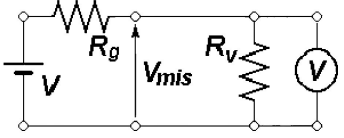
\includegraphics[scale=0.9]{Circuito Misurazione Tensione 2.png}
\end{center}
Risolvendo lo studio teorico del circuito si ottiene l’espressione dell’alterazione inteodotta sia in 
termini assoluti, sia in termini relativi a V. \\
L’alterazione introdotta per la presenza dello strumento viene chiamata errore di perturbazione o 
errore di consumo. L'errore di consumo diminuisce all'aumentare del rapporto Rv / Rg.
\end{document}
